\documentclass[
    11pt,
    spanish,
    a4paper
]{article}
\usepackage[a4paper,left=.4in,right=.4in,top=1in,bottom=1in]{geometry}
\usepackage[utf8]{inputenc}
\usepackage[spanish]{babel}
\usepackage{authoraftertitle}
\usepackage{booktabs}
\usepackage{caption}
\usepackage{float}
\usepackage{graphicx}
\usepackage{listings}
\usepackage{verbatim}

\def\doctype{Trabajo práctico}
\title{Falla por recalentamiento del reactor}
\author{Gonzalo Nahuel Vaca}

\begin{document}

\makeatletter
\begin{titlepage}
	\begin{center}
		\vspace*{1cm}

		\Huge
		\textbf{\doctype}
		\vspace{0.5cm}

		\LARGE
		\@title
		\vspace{0.5cm}

		\textbf{Introducción a los sistemas críticos}

		\vspace{1.5cm}

		\textbf{\@author}

		\vspace{1.5cm}

		
\includegraphics[width=0.8\textwidth]{img/logoFIUBA.pdf}

		\vfill
		Maestría en Sistemas Embebidos\\
		Universidad de Buenos Aires\\
		Argentina\\
		\today
	\end{center}
\end{titlepage}
\makeatother
\newpage

\section{Funcionamiento normal del sistema}

El sistema mantiene la temperatura de un reactor por debajo de un nivel máximo.
En la figura \ref{fig:reactor} se puede observar un diagrama en bloques simplificado.

\begin{figure}[htbp]
	\centering
	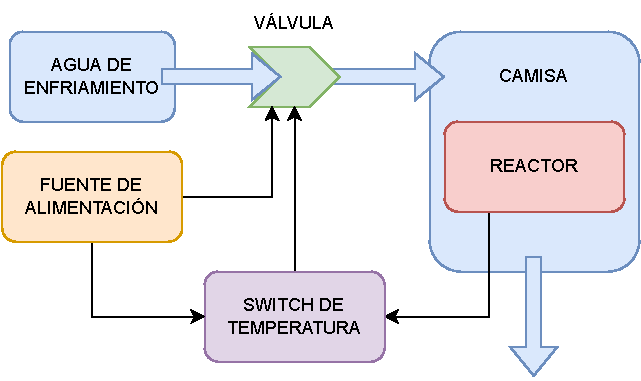
\includegraphics[width=0.8\textwidth]{img/reactor.pdf}
	\caption{Una figura de ejemplo.}
	\label{fig:reactor}
\end{figure}

El funcionamiento esperado es el siguiente:

\begin{enumerate}
	\item El proceso dentro del reactor es exotérmico, esto significa que su temperatura irá en aumento a medida que transcurra el tiempo.
	\item El switch de temperatura detectará que se alcanzó una temperatura máxima tolerable y entregará una señal a la electro-válvula.
	\item La electro-válvula permitirá el paso de agua de refrigeración por la camisa que contiene al reactor.
	\item El flujo de agua refrigerante disminuye la temperatura del reactor.
	\item Cuando la temperatura alcanza un nivel normal el switch envía la señal de cierre a la electro-válvula.
	\item La electro-válvula detiene el flujo de agua refrigerante.
	\item El ciclo vuelve a comenzar.
\end{enumerate}

\section{Metodología de realización de \emph{FEMEA}}

Se decidió adherirse a la norma MIL-STD 1629 del departamento de defensa de los Estados Unidos de Norte América.
En particular, sus criterios de severidad, tasas de falla y probabilidades de detección de fallas.
Para su confección se debe realizar:

\begin{itemize}
	\item{Análisis de modo de falla y efectos (FMEA).}
	\item{Análisis de criticidad.}
\end{itemize}

Como limitación importante es que el análisis solo contempla el \emph{hardware}.

\subsection{FMEA}

Para realizar el \emph{FMEA} se sigue el siguiente procedimiento:

\begin{enumerate}
	\item Definir el sistema.
	\item Construir diagramas en bloques.
	\item Identificar todos los modos potenciales de falla.
	\item Evaluar cada modo potencial de falla y asignar criticidad.
	\item Identificar métodos de detección.
	\item Identificar diseño correctivo.
	\item Identificar los efectos de las acciones correctivas.
	\item Documentar el análisis.
\end{enumerate}

\section{Listado de componentes}

Componentes:

\begin{itemize}
	\item Agua de enfriamiento (CW).
	\item Camisa (C).
	\item Fuente de alimentación (PS).
	\item Reactor (R).
	\item Switch de temperatura (SW).
	\item Válvula (V).
\end{itemize}

En el cuadro \ref{tab:failure} se puede observar un resumen de los modos de falla y su análisis de efectos.

\begin{table}[h]
	\centering
	\caption[Failure mode and effect analysis]{Failure mode and effect analysis}
	\begin{tabular}{c c c c c c c}
		\toprule
		\textbf{Código} & \textbf{Función} & \textbf{Modo} & \textbf{Causa} & \textbf{Efecto}  & \textbf{Criticidad} & \textbf{Comentarios} \\
		\midrule
		CW              & Enfriamiento     & Degradado     & Obstrucción    & Sobretemperatura & III                 &                      \\
		C               & Enfriamiento     & Degradado     & Pérdida        & Sobretemperatura & II                  & Falla                \\
		PS              & Alimentación     & C. abierto    & Fusible        & Sobretemperatura & II                  & Falla                \\
		R               & Producción       & Degradado     & Pérdida        & Catastrófico     & I                   & Falla                \\
		SW              & Control          & Apertura      & Tiristor       & Catastrófico     & I                   & Falla                \\
		V               & Control          & Apertura      & Bobina         & Catastrófico     & I                   & Falla                \\
		\bottomrule
		\hline
	\end{tabular}
	\label{tab:failure}
\end{table}

\section{Conclusiones}

La metodología propicia la reflexión sobre los posibles problemas e invita a desarrollar técnicas de mitigación.

\end{document}